\documentclass{article}


% space between list items
\usepackage{enumitem}
\setlist{nosep}
\setlist[description]{leftmargin=1em, labelindent=0pt, labelsep=0.5em}

% margins
\usepackage[a4paper,left=3cm,right=3cm,top=2cm,bottom=2cm]{geometry}

% Discourage text from running into the margins.
\emergencystretch \textwidth

% prevent widow/orphan lines over the entire document
\usepackage[defaultlines=2,all]{nowidow}

% URL formatting
\usepackage{url}

\usepackage{caption}
\usepackage{nameref}

% automatic intradocument links
\usepackage[colorlinks=false]{hyperref}

% more math commands, like \binom
\usepackage{amsmath}

\usepackage{cleveref}

% Cross-references to main.tex
\usepackage{xr-hyper} % after hyperref

% graphics
\usepackage{graphicx}
\graphicspath{{si-figures}}

% float positioning
\usepackage{float}

% wrapped figures
\usepackage{wrapfig}

% wrapped tables
\usepackage{tabularray}

% supplementary items
\usepackage{newfloat}
\DeclareFloatingEnvironment[name={Supplementary Figure}]{sifigure}
\DeclareFloatingEnvironment[name={Supplementary Table}]{sitable}

% bibliography
\usepackage{natbib}

% Greek letters in text mode
\usepackage{textgreek}

% main typeface
\usepackage{fontspec}
%\setmainfont{Helvetica}
%\setmonofont{Courier}

% 2.0-line spacing
\usepackage{setspace}
\doublespacing

% title and heading typefaces
\usepackage{titlesec}
\titleformat{\section}{\singlespacing\LARGE\raggedright\bfseries}{}{0pt}{}
\titleformat{\subsection}{\singlespacing\Large\raggedright\bfseries}{}{0pt}{}
\titleformat{\subsubsection}{\singlespacing\large\raggedright\bfseries}{}{0pt}{}


\externaldocument{main}


% title
\title{Supplementary Data for ``SEISMIC-RNA: scalable, fully automated RNA structure ensemble analysis with bias correction"}
\author{Matthew F. Allan\textsuperscript{1}, Justin Aruda\textsuperscript{1,2}, and Silvi Rouskin\textsuperscript{1\textdagger}}
\date{
	\textsuperscript{1} Department of Microbiology, Harvard Medical School, Boston, Massachusetts, USA 02115 \\
	\textsuperscript{2} Harvard Program in Biological and Biomedical Sciences, Division of Medical Sciences, Harvard Medical School, Boston, MA, USA 02115 \\
	\textsuperscript{\textdagger} To whom correspondence should be addressed: silvi@hms.harvard.edu \\
}


\begin{document}


\begin{singlespace}
\maketitle
\end{singlespace}


\section{Supplementary Figures}
\label{supp-figures}


\begin{sifigure}[H]
	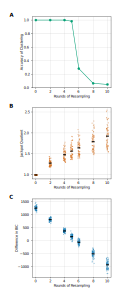
\includegraphics[width=0.619\textwidth]{jackpotting.pdf}
	\caption{\textbf{Jackpotting causes false clusters.} (Continued on next page.)}
	\label{jackpotting}
\end{sifigure}
\addtocounter{sifigure}{-1}
\pagebreak
\begin{sifigure}[H]
	\caption[]{(Continued from previous page.) \textbf{(A)} The fraction of 60 FASTQ files (each of a random 280~nt RNA with 1 structure and 200,000 simulated reads) for which SEISMIC-RNA correctly found 1 cluster as a function of the number of rounds of resampling 200,000 reads with replacement. \textbf{(B)} The distribution of jackpotting quotients for each number of rounds of resampling. Horizontal black bars show means. \textbf{(C)} The distribution of the difference in BIC between 2 clusters and 1 cluster for each number of rounds of resampling. Horizontal black bars show means.}
\end{sifigure}
\pagebreak


\begin{sifigure}[H]
	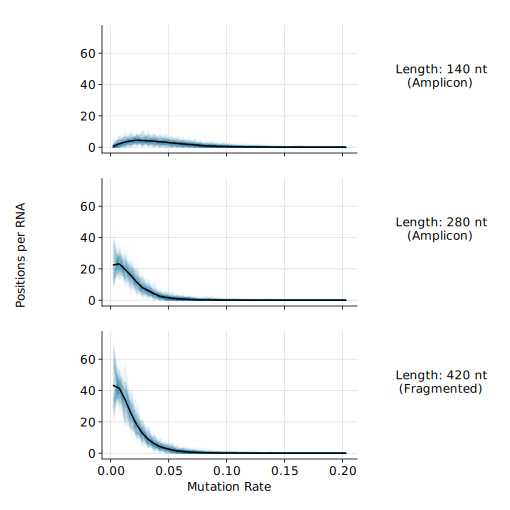
\includegraphics[width=\textwidth]{mus-hist-200000.pdf}
	\caption{\textbf{Histogram of mutation rates using 200,000 reads.} For each reference length, the histogram of the mutation rates on A and C positions for all 240 RNAs with 200,000 simulated reads (transparent blue). The black line shows the average. The bin size for the histogram is 0.005.}
    \label{mus-hist-200000}
\end{sifigure}
\pagebreak


\begin{sifigure}[H]
	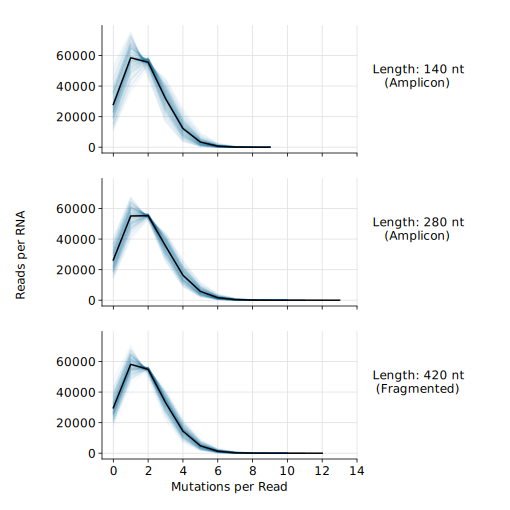
\includegraphics[width=\textwidth]{nmut-hist-200000.pdf}
	\caption{\textbf{Histogram of number of mutated bases per read using 200,000 reads.} For each reference length, the histogram of the number of mutated bases for all 240 RNAs with 200,000 simulated reads (transparent blue). The black line shows the average. The RNAs were simulated to have an average of 2 mutations per read.}
	\label{nmut-hist-200000}
\end{sifigure}
\pagebreak


\begin{sifigure}[H]
	\includegraphics[width=\textwidth]{ncov-200000.pdf}
	\caption{\textbf{Read coverage per position using 200,000 reads.} For each reference length, the number of informative base calls at each position for all 240 RNAs with 200,000 simulated reads (transparent blue). The black line shows the average.}
	\label{ncov-200000}
\end{sifigure}
\pagebreak


\begin{sifigure}[H]
	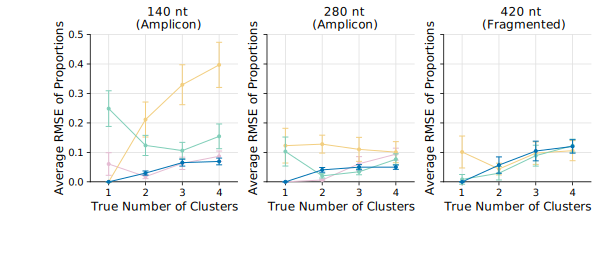
\includegraphics[width=\textwidth]{average-pis-rmse_main-200000.pdf}
	\caption{\textbf{Accuracy of cluster proportions using 200,000 reads.} Average root-mean-square error (RMSE) between the true cluster proportions and those calculated by SEISMIC-RNA, DanceMapper, DRACO, and DREEM for each length of RNA and true number of clusters. Lower RMSEs are more accurate. Error bars show 95\% confidence intervals.}
	\label{average-pis-rmse_main-200000}
\end{sifigure}
\pagebreak


\begin{sifigure}[H]
	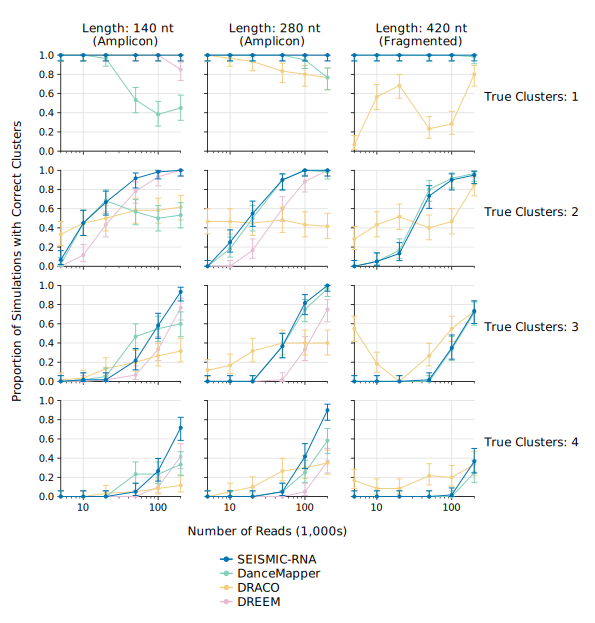
\includegraphics[width=\textwidth]{vs-reads-correct-k-main.pdf}
	\caption{\textbf{Accuracy of number of clusters versus number of reads for each software.} Proportion of simulated FASTQ files for which each piece of software detected the correct number of clusters as a function of number of reads for each reference length and true number of clusters. Higher proportions are more accurate. Error bars show 95\% confidence intervals.}
	\label{vs-reads-correct-k-main}
\end{sifigure}
\pagebreak


\begin{sifigure}[H]
	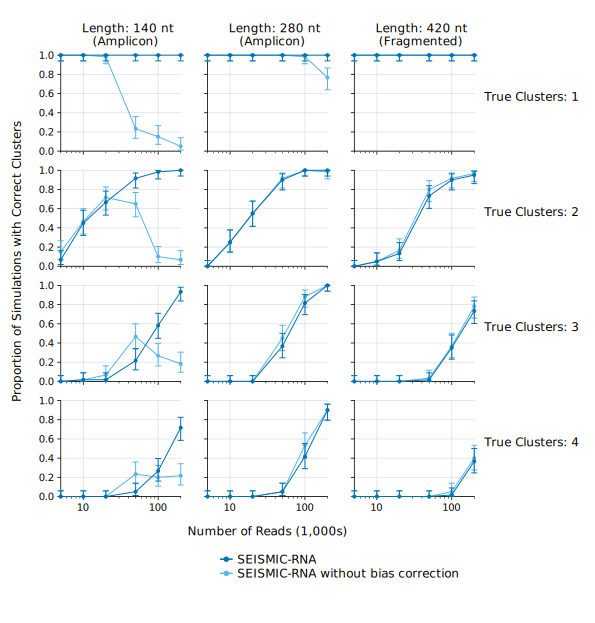
\includegraphics[width=\textwidth]{vs-reads-correct-k-seismic.pdf}
	\caption{\textbf{Accuracy of number of clusters versus number of reads without bias correction.} Proportion of simulated FASTQ files for which SEISMIC-RNA with and without bias correction detected the correct number of clusters as a function of number of reads for each reference length and true number of clusters. Higher proportions are more accurate. Error bars show 95\% confidence intervals.}
	\label{vs-reads-correct-k-seismic}
\end{sifigure}
\pagebreak


\begin{sifigure}[H]
	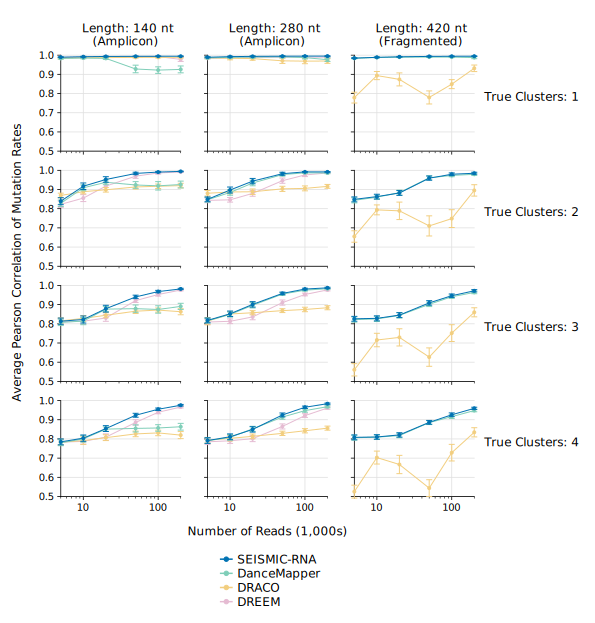
\includegraphics[width=\textwidth]{vs-reads-mus-pcc-main.pdf}
	\caption{\textbf{Accuracy of mutation rates versus number of reads for each software.} Average Pearson correlation between the true mutation rates and the mutation rates detected by each piece of software as a function of number of reads for each reference length and true number of clusters. Higher correlations are more accurate. Error bars show 95\% confidence intervals.}
	\label{vs-reads-mus-pcc-main}
\end{sifigure}
\pagebreak


\begin{sifigure}[H]
	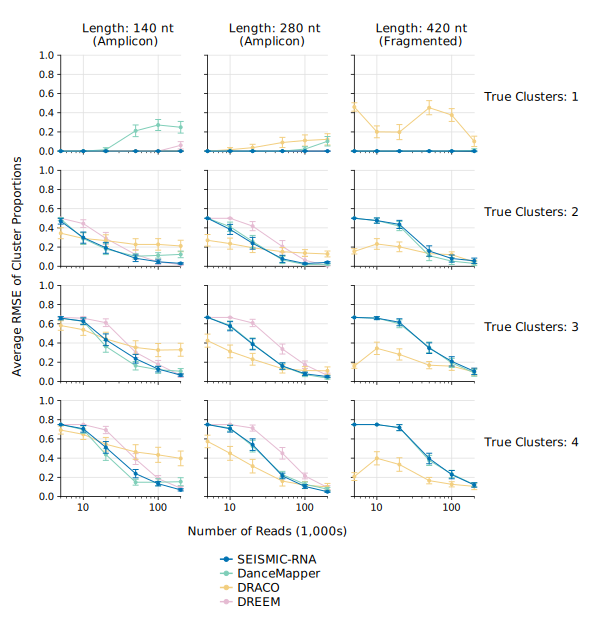
\includegraphics[width=\textwidth]{vs-reads-pis-rmse-main.pdf}
	\caption{\textbf{Accuracy of cluster proportions versus number of reads for each software.} Average root-mean-square error (RMSE) between the true cluster proportions and the cluster proportions detected by each piece of software as a function of number of reads for each reference length and true number of clusters. Lower RMSEs are more accurate. Error bars show 95\% confidence intervals.}
	\label{vs-reads-pis-rmse-main}
\end{sifigure}
\pagebreak


\begin{sifigure}[H]
	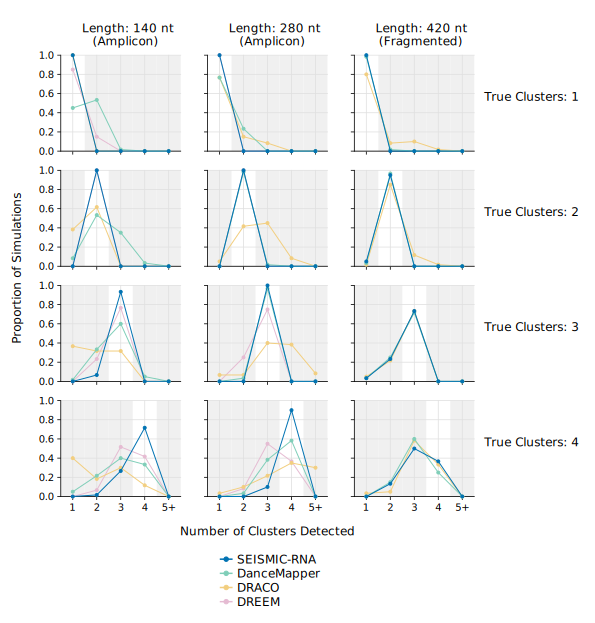
\includegraphics[width=\textwidth]{proportion-each-k-main-200000.pdf}
	\caption{\textbf{Distribution of number of clusters detected using 200,000 reads.} Proportion of simulated FASTQ files for which each piece of software detected each number of clusters for each reference length and true number of clusters.}
	\label{proportion-each-k-main-200000}
\end{sifigure}
\pagebreak


\begin{sifigure}[H]
	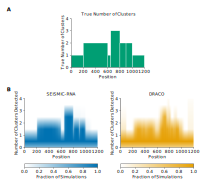
\includegraphics[width=\textwidth]{long-transcript-ks.pdf}
	\caption{\textbf{Number of clusters detected at each position in long transcripts.} \textbf{(A)} Location, length, and number of clusters formed by each ground truth domain in every 1,200~nt RNA. Domains are surrounded by white borders to help distinguish them visually. \textbf{(B)} Fraction of 60 simulated 1,200~nt RNAs for which SEISMIC-RNA and DRACO detected each number of clusters at each position. Cluster numbers are cumulative: e.g. if at position 1, 25\% of RNAs yielded 1 cluster, 50\% yielded 2, and 25\% yielded 3, then the area between 2 and 3 on the y axis (meaning at least 3 clusters) would be 25\% dark, between 1 and 2 (meaning at least 2 clusters) would be 75\% dark, and between 0 and 1 (meaning at least 1 cluster) would be 100\% dark.}
	\label{long-transcript-ks}
\end{sifigure}
\pagebreak


\begin{sifigure}[H]
	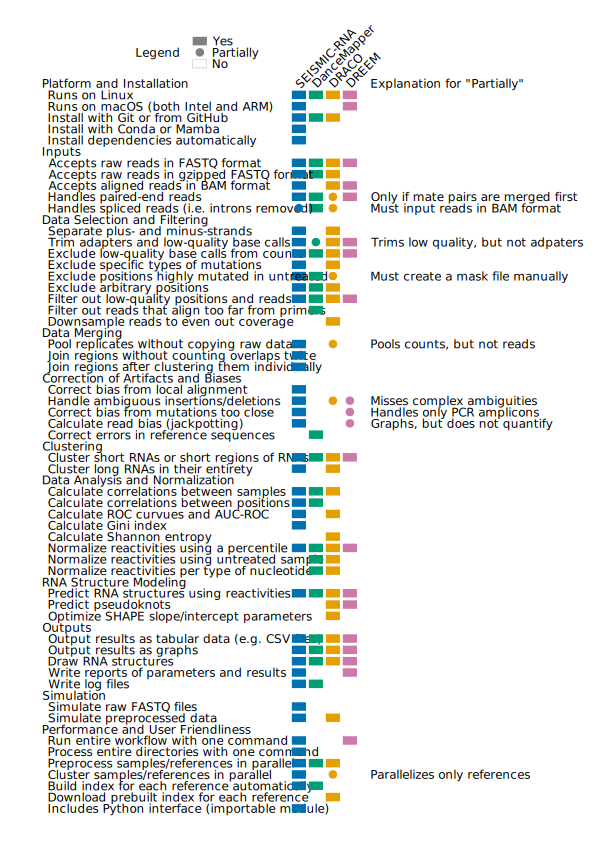
\includegraphics[width=\textwidth]{features.pdf}
	\caption{\textbf{SEISMIC-RNA offers unique features compared to other software.} (Continued on next page.)}
	\label{features}
\end{sifigure}
\addtocounter{sifigure}{-1}
\pagebreak
\begin{sifigure}[H]
	\caption[]{(Continued from previous page.) A list of features supported by each piece of software. For DanceMapper~\cite{Olson2022} and DRACO~\cite{Morandi2021}, this chart includes the features of ShapeMapper~2~\cite{Busan2018} and RNA Framework~\cite{Incarnato2018}, respectively, which are required for preprocessing the data before clustering. For each feature that is ``Partially" supported, an explanation of what specifically is supported is given in the right column.}
\end{sifigure}
\pagebreak


\section{Supplementary Methods}
\label{supp-methods}

\subsection{Converting alignment maps into matrices of relationships}

\subsubsection{Encoding relationships between the read and reference}
\label{relationship-codes}

There are eight types of primary relationships between a base call in the read and the corresponding position in the reference sequence.
These relationships are encoded as bits in an 8-bit (1-byte) integer: \\

\begin{tabular}{ l r r }
\hline
\textbf{Primary Relationship} & \textbf{Binary (8-bit)} & \textbf{Decimal} \\
\hline
Match & 00000001 & 1 \\
Deletion in the read & 00000010 & 2 \\
5' of an Insertion in the read & 00000100 & 4 \\
3' of an Insertion in the read & 00001000 & 8 \\
Substitution to A & 00010000 & 16 \\
Substitution to C & 00100000 & 32 \\
Substitution to G & 01000000 & 64 \\
Substitution to T & 10000000 & 128 \\
\hline
\end{tabular} \\

Ambiguous relationships can be represented via the bitwise OR of primary relationships.
A relationship code signifies that the relationship could be any of the bits of which it is made.
For example, if a base call in the read has a low quality score, then it is assumed that the true base in the read could be any of the four bases.
If the base at the corresponding position in the reference is an A, then the base call in the read could be either a match (if it were truly an A) or a substitution to C, G, or T (if it were truly any of those bases).
Hence, the relationship code is 11100001: the bitwise OR of match and substitutions to C, G, and T.
There are several common ambiguous relationships: \\

\begin{tabular}{ l r r }
\hline
\textbf{Ambiguous Relationship} & \textbf{Binary (8-bit)} & \textbf{Decimal} \\
\hline
Paired-end mates contradict each other & 00000000 & 0 \\
Ambiguously Match or Deletion & 00000011 & 3 \\
Ambiguously Match or 5' of an Insertion & 00000101 & 5 \\
Ambiguously Match or 3' of an Insertion & 00001001 & 9 \\
Read is low-quality or N; reference is T & 01110001 & 113 \\
Read is low-quality or N; reference is G & 10110001 & 177 \\
Read is low-quality or N; reference is C & 11010001 & 209 \\
Read is low-quality or N; reference is A & 11100001 & 225 \\
Reference is N (ambiguous/unknown) & 11110001 & 241 \\
The read does not cover the position & 11111111 & 255 \\
\hline
\end{tabular} \\

The relationship between a base in the reference and a base in the read is determined as follows:
\begin{enumerate}
    \item If the reference base is not A, C, G, or T, then the relationship code is 11110001.
    \item Otherwise, if the read base is not A, C, G, or T; or if its quality score is below the minimum, then the relationship code is 11110001 minus the bit corresponding to a substitution to the reference base (from the table above).
    \item Otherwise, if the read base matches the reference base, then the relationship code is 00000001.
    \item Otherwise, the relationship code is a substitution to the base in the read (from the table above).
\end{enumerate}

\subsubsection{Storing mutational profiling data in a sparse structure}

In chemical probing experiments, mutations occur at low rates.
Consequently, a sparse data structure is much more efficient at storing mutational profiling data than a full matrix of reads by positions -- especially when the reference is much longer than the reads.

The positions of the ends of the reads are stored as two NumPy arrays~\cite{Harris2020} -- one for the 5' and one for the 3' ends.
Each row in the array corresponds to one read in a batch, and each column corresponds to one segment in the read: single-end reads have one segment, paired-end reads have two. 
Additionally, using \verb|seismic join| causes the arrays to be concatenated horizontally, increasing the number of segments per read.

The relationships between the read and reference are stored as a three-level data structure:
\begin{enumerate}
    \item The first level is a Python \verb|dict| in which each key is a position in the reference sequence and each value is a Python \verb|dict|.
    \item In the second level, for each Python \verb|dict| each key is a relationship code (see ``\nameref{relationship-codes}") and each value is a NumPy array~\cite{Harris2020}.
    \item In the third level, each NumPy array contains the indexes of the reads in the batch that have the relationship code (second level) at the position (first level).
\end{enumerate}

\subsubsection{Converting aligned reads into vectors of relationships}
\label{relationship-vector}

Each alignment map is collated and converted into a SAM file using SAMtools~\cite{Danecek2021}.
Each read in the SAM file is then parsed to generate a vector of relationships to the reference sequence as follows:
\begin{enumerate}
    \item Initialize the position in the read to 1 and the position in the reference to the mapping position in the SAM file~\cite{Li2009}.
    \item Initialize the 5' and 3' ends of the read to 1 and the read length (in read coordinates).
    \item Initialize empty lists of the 5' and 3' ends of segments in the read.
    \item Initialize an empty map of positions to their relationship codes (only for non-matches, to save effort).
    \item Initialize an empty list of insertions and deletions (``indels").
    \item Loop over each operation in the CIGAR string~\cite{Li2009} and act based on the type of operation:
    \begin{description}
        \item[Match or Substitution (M/X/=):] For the length of the operation:
        \begin{enumerate}
            \item Use the base in the reference, the base in the read, and the read quality to encode the relationship between the read and the reference (for details, see ``\nameref{relationship-codes}").
            \item Map the current position in the reference to the relationship if it is not a match.
            \item Increment the positions in both the read and reference.
        \end{enumerate}
        \item[Deletion (D):] For the length of the operation:
        \begin{enumerate}
            \item Map the current position in the reference to the deletion relationship (for details, see ``\nameref{relationship-codes}".
            \item Add a deletion to the list of indels.
            \item Increment the position in the reference.
        \end{enumerate}
        \item[Insertion (I):] For the length of the operation:
        \begin{enumerate}
            \item Add an insertion to the list of indels. (Do not map the reference position to an insertion yet; that will happen later.)
            \item Increment the position in the read.
        \end{enumerate}
        \item[Intron or other Skipped Region (N):] This is the end of a contiguous segment:
        \begin{enumerate}
            \item Add the current position in the reference to the list of segment 3' ends.
            \item Advance the reference position by the length of the operation.
            \item Add the new position in the reference to the list of segment 5' ends (so that a new segment can begin).
        \end{enumerate}
        \item[Soft Clip (S):] The 5' or 3' end must be clipped off:
        \begin{enumerate}
            \item Determine the location of the soft clip:
            \begin{description}
                \item[5' end:] Increase the 5' end of the read by the length of the operation (to clip off the first bases).
                \item[3' end:] Decrease the 3' end of the read by the length of the operation (to clip off the last bases).
                \item[Otherwise:] The location is invalid. Raise an error.
            \end{description}
            \item Increase the position in the read by the length of the operation.
        \end{enumerate}
        \item[Otherwise:] The operation is not supported. Raise an error.
    \end{description}
    \item Add any insertions to the map of positions to relationships. Insertions must be added last because they can overlap other types of relationships. For each insertion:
    \begin{enumerate}
        \item Determine which reference position to mark: the 3' (default) or 5' side of the insertion. Each insertion is located between two positions in the reference; only one is marked to avoid double-counting. If marking the 5' side, use the code 00000100; if the 3' side, use 00001000 (for an explanation, see ``\nameref{relationship-codes}").
        \item If the position to be marked already appears in the map because it has another mutation, then add the insertion code on top of the existing relationship code using bitwise OR. For example, if the position 3' of an insertion were already a substitution to T (10000000), then the result would be 10001000 after marking the insertion.
    \end{enumerate}
    \item Mark ambiguous indels (for details, see ``\nameref{ambiguous-indels}").
    \item Determine the positions of the 5' and 3' ends of the read's footprint in the reference.
    Clip a user-specified number of bases $n$ from both ends of the reference to counteract the bias against mutations near the ends of reads that happens during local alignment (for an explanation, see ``\nameref{seismic-relate}" in the \nameref{methods}):
    \begin{enumerate}
        \item Set the 5' end to the smaller of
        \begin{itemize}
            \item the read's mapping position in the SAM file plus $n$
            \item the reference length plus 1
        \end{itemize}
        \item Set the 3' end to the larger of
        \begin{itemize}
            \item the last position reached in the reference minus $n$
            \item 0
        \end{itemize}
    \end{enumerate}
    \item Prepend the 5' end of the read's footprint in the reference to the the list of segment 5' ends -- it begins the first segment of the read. Append the 3' end of the read's footprint in the reference to the list of segment 3' ends -- it ends the last segment of the read.
    \item Remove from the relationship map any positions that are no longer contained in any segment after clipping $n$ positions from both ends.
\end{enumerate}

\subsubsection{Merging the relationships of paired-end reads}

If the reads are paired-end and two mates are properly paired, then after both mates are processed as described in ``\nameref{relationship-vector}", several more steps are required to merge them:
\begin{enumerate}
    \item Ensure that one mate (can be either 1 or 2) aligns in the forward orientation and the other aligns in the reverse orientation (if not, raise an error).
    \item If (optionally) removing overhangs of mates that dovetail:
    \begin{enumerate}
        \item For each segment of the reverse-aligned read, if its 5' end extends beyond the forward-aligned read, then trim it so that it is flush with the 5' end of the forward-aligned read. Remove any position-relationship mappings in the trimmed part.
        \item For each segment of the forward-aligned read, if its 3' end extends beyond the reverse-aligned read, then trim it so that it is flush with the 3' end of the reverse-aligned read. Remove any position-relationship mappings in the trimmed part.
    \end{enumerate}
    \item Concatenate the segment 5' and 3' end positions from both mates, putting the segment(s) of the forward-aligned mates first and those of the reverse-aligned mates last.
    \item Initialize a merged map of positions to relationships. For each position that occurs in the position-relationship map of at least one mate:
    \begin{enumerate}
        \item Find the relationship at that position in the forward-aligned mate.
        \begin{itemize}
            \item If the position is in the forward mate's map (because it is a mutation), then use the relationship code from the map.
            \item If the position is not in the map but lies within any segment of the forward mate, then the position is a match (code 00000001).
            \item Otherwise, the position is not covered by the mate (code 11111111).
        \end{itemize}
        \item Find the relationship at that position in the reverse-aligned mate using the same procedure.
        \item Take the bitwise AND of the forward and reverse mates' relationship codes. This limits the possible relationships to those on which the mates agree. It also lets one mate compensate for low quality or lack of coverage in the other mate. For example, if the reference base was an A, mate 1 was low quality (code 11100001), and mate 2 was a high-quality substitution to T (code 10000000), then the bitwise AND would be a substitution to T.
        \item If the bitwise AND is not a match (code 00000001), then add it to the merged map of positions to relationships.
    \end{enumerate}
\end{enumerate}


\subsubsection{Detecting and labeling ambiguous insertions and deletions}
\label{ambiguous-indels}

When insertions and deletions (collectively ``indels") occur in repetitive regions or next to substitutions or low-quality base calls, it can be impossible to assign them unambiguously to one position.
For example, if the reference sequence were AGCCTA and a read were AGCTA, then it would be clear that one C had been deleted, but impossible to determine which.
Aligners like Bowtie 2~\cite{Langmead2012} will arbitrarily choose a location for the indel, but it may not be the true location.
To avoid labeling the wrong positions as indels, all indels with ambiguous locations must be identified and labeled.

First, all indels and their locations are listed during the relationship encoding process (for details, see ``\nameref{relationship-vector}".
Each indel keeps track of two positions:
\begin{description}
    \item[Inline position:] The position in the sequence that contains the base. It must be \textbf{unique} among indels.
    \begin{description}
        \item[For a deletion,] this is the position in the \textbf{reference} of the base that has been deleted from the read.
        \item[For an insertion,] this is the position in the \textbf{read} of the base that has been inserted into the read.
    \end{description}
    \item[Lateral position:] The position in the sequence that is missing the base. Because the base is absent, it does not correspond to a position in the sequence, so the position of the existing base on either side must be used instead (hence ``lateral" position). By convention the position of the base immediately 3' of the missing base is used as the lateral position. Adjacent indels will have the \textbf{same} lateral position.
    \begin{description}
        \item[For a deletion,] this is the position in the \textbf{read} of the base immediately 3' of the deletion.
        \item[For an insertion,] this is the position in the \textbf{reference} of the base immediately 3' of the insertion.
    \end{description}
\end{description} 

Indels of the same type (namely, insertion or deletion) that do not have another indel of the other type between them are grouped into ``pods".
Indels do not need to occur at consecutive positions to be in the same pod: there just needs to be no indel of the other type between them.
For example, suppose a read had deletions at reference positions 20, 45, and 103; and insertions at positions 68 and 72.
It would have three pods:
\begin{enumerate}
    \item Deletions 20 and 45
    \item Insertions 68 and 72
    \item Deletion 103
\end{enumerate}

The algorithm discovers all possible ways the indels could move without changing the read-reference relationships (hence why the locations are ambiguous) under the constraint that two pods never move past each other.
(This constraint is necessary for computational tractability because it allows processing each pod independently; in practice it almost never makes a difference in the result.)
It works as follows, in two major phases:
\begin{enumerate}
    \item In the first phase, all indels are moved as far as possible in the 5' direction.
    To avoid one pod blocking another's movement, the 5'-most pod must be moved first.
    For each pod in order from 5' to 3':
    \begin{enumerate}
        \item Ensure the indels in the pod are sorted from 5' to 3'.
        \item Given that the pod contains $n$ indels, initialize a pointer $i$ to indel $n$ (the 3'-most indel).
        The 3'-most indel must be moved first in order to handle multi-base deletions.
        \item While $i \ge 1$ (the 5'-most indel):
        \begin{enumerate}
            \item Compute a set of three trial positions to which to try moving indel $i$:
            \begin{description}
                \item[Trial inline position:] Set it to one position 5' of the indel's current inline position.
                Because inline positions must be unique, keep moving it one position 5' until it does not match the inline position of any other indel.
                This prevents the trial inline position from matching the inline position of any adjacent indel.
                \item[Trial lateral position:] Set it to the position 5' of the indel's current lateral position.
                \item[Trial swap position:] The position in the sequence that is missing the base with which the indel is trying to swap.
                Set it to the lateral position on the 5' side of the indel.
            \end{description}
            \item Check whether the trial move is valid, if all of the following are true:
            \begin{itemize}
                \item The trial inline position is within the bounds of the reference sequence (if a deletion) or read sequence (if an insertion).
                \item The move would not cause the indel to collide with any indel in an adjacent pod, based on the trial lateral position.
                \item The relationships would be consistent before and after moving the indel:
                \begin{enumerate}
                    \item Find the base with which the indel would swap during the move (located at the trial swap position).
                    \begin{description}
                        \item[For a deletion:] the base in the read immediately 5' of the site of the deletion.
                        \item[For an insertion:] the base in the reference immediately 5' of the site of the insertion.
                    \end{description}
                    \item Find the base at the current inline position.
                    \begin{description}
                        \item[For a deletion:] the base in the reference that is deleted from the read.
                        \item[For an insertion:] the base that is inserted into the read.
                    \end{description}
                    \item Find the base at the trial inline position.
                    \begin{description}
                        \item[For a deletion:] the base in the reference that would be marked as deleted if the deletion moved.
                        \item[For an insertion:] the base in the read that would be marked as inserted if the insertion moved.
                    \end{description}
                    \item Using the method in ``\nameref{relationship-codes}", compute the relationships between the swap base and
                    \begin{itemize}
                        \item the base at the current inline position
                        \item the base at the trial inline position
                    \end{itemize}
                    \item The relationships are consistent if either of the following is true:
                    \begin{itemize}
                        \item The relationship codes have at least one bit in common (the bitwise AND is not zero).
                        \item Both relationships are substitutions to any base (not necessarily to the same base).
                    \end{itemize}
                \end{enumerate}
            \end{itemize}
            \item If the move is valid, then move the indel to the trial position.
            \begin{description}
                \item[For a deletion:] The deletion moves from the current inline position to the trial inline position in the reference.
                Meanwhile, the swap base in the read moves from the trial inline position to the the current inline position.
                \begin{enumerate}
                    \item To the current inline position, mark (with bitwise OR) the relationship between it and the swap base, which moves to that position.
                    \item To the trial inline position, mark (with bitwise OR) the code for the deletion (00000010), which moves to that position.
                    \item Move the deletion's inline and lateral positions to the trial positions.
                \end{enumerate}
                \item[For an insertion, if marked on the 5' side:] The insertion moves from the current inline position to the trial inline position in the read.
                Meanwhile, the swap base in the reference moves from the trial inline position to the the current inline position.
                \begin{enumerate}
                    \item Move the insertion's inline and lateral positions to the trial positions.
                    \item On the 5' side after the move, mark (with bitwise OR) the code for the insertion.
                    \item On the 3' side after the move, mark (with bitwise OR) the relationship between the current inline position and the swap base.
                    If that relationship is a match, then mark it only if that position is not immediately 5' of another insertion.
                \end{enumerate}
                \item[For an insertion, if marked on the 3' side:] The insertion moves from the current inline position to the trial inline position in the read.
                Meanwhile, the swap base in the reference moves from the trial inline position to the the current inline position.
                \begin{enumerate}
                    \item On the 3' side before the move, mark (with bitwise OR) the relationship between the read and reference at that position.
                    (If that relationship is a match, then it will have been marked as 3' of an insertion, not a match, so because the insertion is moving it must now also be marked as a match.)
                    \item Move the insertion's inline and lateral positions to the trial positions.
                    \item On the 3' side after the move, mark (with bitwise OR) the codes for the insertion and for the relationship between the current inline position and the swap base (if it's not a match).
                \end{enumerate}
            \end{description}
            \item If any indel moved through another indel, then re-sort the indels in the pod so that they are still in 5' to 3' order.
            \item If the move was not valid, then decrement $i$.
            This means that this indel has no more valid moves in the 5' direction, so the next indel must be tried.
        \end{enumerate}
    \end{enumerate}
    \item In the second phase, all indels are moved as far as possible in the 3' direction.
    Unlike in the first phase, also detect all possible permutations of indels as they move.
    It works the same way as the first phase, with two exceptions:
    \begin{itemize}
        \item Movements and sorting are in the opposite direction: all 5' and 3' labels in the first phase are swapped.
        \item If an indel is moved successfully, then adjust $i$ to point at that indel again, rather than keeping $i$ unchanged.
        For example, if $i$ were 1 and the indel in 1st place in the pod wound up in 2nd place after it moved and the indels were re-sorted, then adjust $i$ to 2.
        This adjustment is necessary to consider all possible permutations of indels in the second phase, which searches more exhaustively than the first phase.
    \end{itemize}
\end{enumerate}


\subsection{Correcting bias due to underrepresentation of reads with nearby mutations}
\label{bias-correction-algorithm}

Let $N$ reads from $K$ clusters align to a reference sequence of length $J$.
Let the proportion of reads whose 5' and 3' ends align, respectively, to coordinates $a$ and $b$ ($1 \le a \le b \le J$) be $\eta_{ab}$ (assuming these proportions are equal for all clusters). Let the mutation rate of base $j$ ($1 \le j \le J$) in cluster $k$ ($1 \le k \le K$) be $\mu_{jk}$.
Let the proportion of cluster $k$ in the ensemble be $\pi_k$.
To express these quantities as probabilities, let $C_k$ be the event that a read comes from cluster $k$; let $E_{ab}$ be the event that a read aligns with 5' and 3' coordinates $a$ and $b$, respectively; let $S_j$ be the event that a read contains position $j$ (i.e. its alignment coordinates $a$ and $b$ satisfy $1 \le a \le j \le b \le J$); let $M_j$ be the event that a read has a mutation at position $j$; and let $G_g$ be the event that a read has no two mutations separated by fewer than $g$ non-mutated bases.

\subsubsection{Deriving mutation rates of reads with no two mutations too close}
\label{calc_p_mut_noclose}

In terms of these events, the total mutation rates ($\mu_{jk}$) are $P(M_j | S_j C_k)$, i.e. the probability that a read would have a mutation at position $j$ given that it contained position $j$ and came from cluster $k$; and the observable mutation rates ($m_{jk}$) are $P(M_j | S_j C_k G_g)$, i.e. the probability that a read would have a mutation at position $j$ given that it contained position $j$, came from cluster $k$, and had no two mutations closer than $g$ bases.
Using these definitions and Bayes' theorem yields a probabilistic formula for $m_{jk}$:
$$m_{jk} = P(M_j | S_j C_k G_g) = P(M_j | S_j C_k) \frac{P(G_g | S_j M_j C_k)}{P(G_g | S_j C_k)} = \mu_{jk} \frac{P(G_g | S_j M_j C_k)}{P(G_g | S_j C_k)}$$

The term $P(G_g | S_j C_k)$ is the probability that a read would have no two mutations closer than $g$ bases given that it contained position $j$ and came from cluster $k$.
It can be computed using $P(G_g | E_{ab} C_k)$ (abbreviated $d_{abk}$): the probability that a read would contain no two mutations closer than $g$ bases given that its 5' and 3' coordinates are $a$ and $b$, respectively ($1 \le a \le b \le J$), and that it came from cluster $k$.
If position $b$ were mutated (probability $\mu_{bk}$), then the read would contain no two mutations closer than $g$ bases if and only if none of the $g$ bases preceding $b$ (i.e. positions $b - g$ to $b - 1$, inclusive) were mutated (probability $\prod_{j'=\max(b-g, a)}^{b-1}(1 - \mu_{j'k})$, abbreviated $w_{\max(b-g, a),b-1,k}$) and no two mutations between positions $a$ and $b - (g + 1)$, inclusive, were too close (probability $d_{a,\max(b-(g+1), a),k})$).
If position $b$ were not mutated (probability $1 - \mu_{bk}$), then the read would contain no two mutations closer than $g$ bases if and only if no mutations between positions $a$ and $b - 1$, inclusive, were too close (probability $d_{a,\max(b-1,a),k}$).
These two possibilities generate a recurrence relation:
$$d_{abk} = \mu_{bk} w_{\max(b-g, a),b-1,k} d_{a,\max(b-(g+1), a),k} + (1 - \mu_{bk}) d_{a,\max(b-1,a),k}$$
The base case is $d_{abk} = 1$ when $a = b$ because such a read would contain one position and thus be guaranteed to have no two mutations too close.
Then, $P(G_g | S_j C_k)$ is the average of $d_{abk}$ over every read that contains position $j$, weighted by the proportions $\eta_{ab}$:
$$P(G_g | S_j C_k) = \frac{\sum_{a=1}^{j}\sum_{b=j}^{J}\eta_{ab}d_{abk}}{\sum_{a=1}^{j}\sum_{b=j}^{J}\eta_{ab}}$$

The term $P(G_g | S_j M_j C_k)$ is the probability that a read would have no two mutations too close given that it contained a mutation at position $j$ and came from cluster $k$.
It can be computed using $P(G_g | M_j E_{ab} C_k)$ (abbreviated $f_{abjk}$): the probability that a read would contain no two mutations too close given that position $j$ is mutated ($1 \le a \le j \le b \le J$), that its 5' and 3' coordinates are $a$ and $b$ (respectively), and that it came from cluster $k$.
Because position $j$ is mutated, having no two mutations too close requires that none of the $g$ bases on both sides of position $j$ be mutated.
The probability that none of the preceding $g$ positions ($j - g$ to $j - 1$) is mutated is $w_{\max(j-g,a),j-1,k}$, while that of the following $g$ positions ($j + 1$ to $j + g$) is $w_{j+1,\min(j+g,b),k}$.
Upstream of the $g$ bases flanking position $j$ (i.e. positions $a$ to $j - (g + 1)$), the probability that no two mutations are too close is $d_{a,\max(j-(g+1),a),k}$; downstream (i.e. positions $j + (g + 1)$ to $b$), the probability is $d_{\min(j+(g+1),b),b,k}$.
Since mutations in these four sections are independent, the probability that the read contains no two mutations too close is the product:
$$f_{abjk} = d_{a,\max(j-(g+1),a),k} w_{\max(j-g,a),j-1,k} w_{j+1,\min(j+g,b),k} d_{\min(j+(g+1),b),b,k}$$
Then, $P(G_g | S_j M_j C_k)$ is the average of $f_{abjk}$ over every read that contains position $j$, weighted by the proportions $\eta_{ab}$.
$$P(G_g | S_j M_j C_k) = \frac{\sum_{a=1}^{j}\sum_{b=j}^{J}\eta_{ab} f_{abjk}}{\sum_{a=1}^{j}\sum_{b=j}^{J}\eta_{ab}}$$

Combining the above results yields an explicit formula for $m_{jk}$:
$$m_{jk} = \mu_{jk} \frac{\sum_{a=1}^{j}\sum_{b=j}^{J}\eta_{ab} f_{abjk}}{\sum_{a=1}^{j}\sum_{b=j}^{J}\eta_{ab}d_{abk}}$$

\subsubsection{Deriving end coordinate proportions of reads with no two mutations too close}
\label{calc_p_ends_noclose}

The total proportions ($\eta_{ab}$) of reads aligned to 5' and 3' coordinates $a$ and $b$, respectively, are $P(E_{ab})$; and the proportions of reads with no two mutations too close that align with coordinates $a$ and $b$ ($e_{abk}$) are $P(E_{ab} | G_g C_k)$.
Using these definitions and Bayes' theorem yields a probabilistic formula for $e_{abk}$:
$$e_{abk} = P(E_{ab} | G_g C_k) = P(G_g | E_{ab} C_k) \frac{P(E_{ab} | C_k)}{P(G_g | C_k)} = d_{abk} \frac{\eta_{ab}}{P(G_g | C_k)}$$

Note that, while reads are assumed to come from the same distribution of coordinates ($\eta_{ab}$) regardless of their cluster $k$, the observable distribution of coordinates ($e_{abk}$) varies by cluster because $d_{abk}$ and $P(G_g | C_k)$ depend on $k$.
The term $P(G_g | C_k)$ is the probability that a read would have no two mutations too close given that it came from cluster $k$.
It can be computed as an average of $P(G_g | E_{ab} C_k)$ (i.e. $d_{abk}$) over all coordinates $a$ and $b$ (such that $1 \le a \le b \le J$), weighted by the proportion of each coordinate, $P(E_{ab})$ (i.e. $\eta_{ab}$):
$$P(G_g | C_k) = \frac{\sum_{a=1}^{J} \sum_{b=a}^{J} \eta_{ab} d_{abk}}{\sum_{a=1}^{J} \sum_{b=a}^{J} \eta_{ab}} = \sum_{a=1}^{J} \sum_{b=a}^{J} \eta_{ab} d_{abk}$$
This expression is already normalized because $\sum_{a=1}^{J} \sum_{b=a}^{J} \eta_{ab} = 1$, by definition.

Combining the above results yields an explicit formula for $e_{abk}$:
$$e_{abk} = \frac{\eta_{ab} d_{abk}}{\sum_{a'=1}^{J} \sum_{b'=a'}^{J} \eta_{a'b'} d_{a'b'k}}$$

\subsubsection{Deriving cluster proportions of reads with no two mutations too close}
\label{calc_p_clust_noclose}

The proportion of total reads in cluster $k$ is $\pi_k = P(C_k)$.
The proportion among only reads with no two mutations closer than $g$ bases is
$$p_k = P(C_k | G_g) = P(G_g | C_k) \frac{P(C_k)}{P(G_g)} = \pi_k \frac{\sum_{a=1}^{J} \sum_{b=a}^{J} \eta_{ab} d_{abk}}{P(G_g)}$$
The term $P(G_g)$ is the probability that a read from any cluster would have no two mutations closer than $g$ bases and can be solved for by leveraging that the cluster proportions ($p_k$) must sum to 1:
$$1 = \sum_{k=1}^{K} p_k = \sum_{k=1}^{K} \pi_k \frac{\sum_{a=1}^{J} \sum_{b=a}^{J} \eta_{ab} d_{abk}}{P(G_g)} = \frac{1}{{P(G_g)}} \sum_{k=1}^{K} \pi_k \sum_{a=1}^{J} \sum_{b=a}^{J} \eta_{ab} d_{abk}$$
$$P(G_g) = \sum_{k=1}^{K} \pi_k \sum_{a=1}^{J} \sum_{b=a}^{J} \eta_{ab} d_{abk}$$
The result is an explicit formula for $p_k$:
$$p_k = \frac{\pi_k \sum_{a=1}^{J} \sum_{b=a}^{J} \eta_{ab} d_{abk}}{\sum_{k'=1}^{K} \pi_{k'} \sum_{a=1}^{J} \sum_{b=a}^{J} \eta_{ab} d_{abk'}}$$

\subsubsection{Solving total mutation rates and cluster and coordinate proportions}
\label{calc_params}

The observed mutation rates ($m_{jk}$), end coordinate proportions ($e_{abk}$), and cluster proportions ($p_k$) can be calculated as weighted averages over the $N$ reads with no two mutations too close:
$$m_{jk} = \frac{\sum_{i=1}^{N} z_{ik} x_{ij}}{\sum_{i=1}^{N} z_{ik} s_{ij}}$$
$$e_{abk} = \frac{\sum_{i=1}^{N} z_{ik} y_{abi}}{\sum_{i=1}^{N} z_{ik}}$$
$$p_k = \frac{\sum_{i=1}^{N} z_{ik}}{N}$$
where $s_{ij}$ is $1$ if read $i$ contains position $j$, otherwise $0$; $x_{ij}$ is $1$ if read $i$ has a mutation at position $j$, otherwise $0$; $y_{abi}$ is $1$ if read $i$ aligns to coordinates $a$ and $b$, otherwise $0$; and $z_{ik}$ is the probability that read $i$ came from cluster $k$.

The original parameters $\mu_{jk}$, $\eta_{abk}$, and $\pi_k$ can be solved by setting the two formulae each for $m_{jk}$, $e_{abk}$, and $p_k$ equal to each other, creating a system of equations:
$$\mu_{jk} \frac{\sum_{a=1}^{j}\sum_{b=j}^{J}\eta_{ab} f_{abjk}}{\sum_{a=1}^{j}\sum_{b=j}^{J}\eta_{ab}d_{abk}} = m_{jk} = \frac{\sum_{i=1}^{N} z_{ik} x_{ij}}{\sum_{i=1}^{N} z_{ik} s_{ij}}$$
$$\eta_{ab} \frac{d_{abk}}{\sum_{a'=1}^{J} \sum_{b'=a'}^{J} \eta_{a'b'} d_{a'b'k}} = e_{ab} = \frac{\sum_{i=1}^{N} z_{ik} y_{abi}}{\sum_{i=1}^{N} z_{ik}}$$
$$\pi_k \frac{\sum_{a=1}^{J} \sum_{b=a}^{J} \eta_{ab} d_{abk}}{\sum_{k'=1}^{K} \pi_{k'} \sum_{a=1}^{J} \sum_{b=a}^{J} \eta_{ab} d_{abk'}} = p_k = \frac{\sum_{i=1}^{N} z_{ik}}{N}$$
Solving this entire system at once has proven computationally impractical for all but extremely short sequences.
A more feasible approach is to first solve for $\mu_{jk}$ given an initial guess for $\eta_{ab}$, next solve for $\eta_{ab}$ given the updated $\mu_{jk}$, then solve for $\pi_k$ given the updated $\mu_{jk}$ and $\eta_{ab}$, and iterate until all three sets of parameters converge.

Even assuming every $\eta_{ab}$ is a constant, these equations are still too complex to solve for $\mu_{jk}$ analytically because $d_{abk}$ and $f_{abjk}$ also depend on $\mu_{jk}$ (as well as on other $\mu$ variables).
Thus, every $\mu_{jk}$ is solved for numerically by rearranging each equation to
$$\mu_{jk} \frac{\sum_{a=1}^{j}\sum_{b=j}^{J}\eta_{ab} f_{abjk}}{\sum_{a=1}^{j}\sum_{b=j}^{J}\eta_{ab}d_{abk}} - m_{jk} = 0$$
and applying the Newton-Krylov method~\cite{Knoll2004} implemented in SciPy~\cite{Virtanen2020}.
This method requires an initial guess for $\mu_{jk}$; if that guess is similar to the eventual solution, the algorithm will run faster.
When clustering with the EM algorithm (see ``\nameref{em-clustering}"), every iteration except the first uses the $\mu_{jk}$ from the previous iteration as the initial guess, since consecutive iterations tend to have similar parameters.
In all other cases, the biased mutation rates ($m_{jk}$) are used, as they tend to be similar to $\mu_{jk}$ unless the mutation rates are large.

Once every $\mu_{jk}$ has been solved for, every $\eta_{ab}$ can be updated.
Because $d_{abk}$ does not depend on $\eta_{ab}$ (except indirectly through the $\mu_{jk}$ parameters, which are now assumed to be constants), each equation can be rearranged to
$$\eta_{ab} = \frac{e_{ab}}{d_{abk}} \sum_{a'=1}^{J} \sum_{b'=a'}^{J} \eta_{a'b'} d_{a'b'k}$$
Leveraging that $\sum_{a=1}^{J} \sum_{b=a}^{J} \eta_{ab} = 1$, by definition, leads to
$$\sum_{a=1}^{J} \sum_{b=a}^{J} \frac{e_{ab}}{d_{abk}} \sum_{a'=1}^{J} \sum_{b'=a'}^{J} \eta_{a'b'} d_{a'b'k} = 1$$
$$\sum_{a'=1}^{J} \sum_{b'=a'}^{J} \eta_{a'b'} d_{a'b'k} = \frac{1}{\sum_{a=1}^{J} \sum_{b=a}^{J} \frac{e_{ab}}{d_{abk}}}$$
and finally a closed-form expression for each $\eta_{ab}$ given $\mu_{jk}$ (and hence $d_{abk}$) and $e_{abk}$:
$$\eta_{ab} = \frac{\frac{e_{ab}}{d_{abk}}}{\sum_{a'=1}^{J} \sum_{b'=a'}^{J} \frac{e_{a'b'}}{d_{a'b'k}}}$$
This equation should theoretically yield the same value of $\eta_{ab}$ for every $k$.
In practice, the values will differ due to inexactness in floating-point arithmetic.
Thus, the consensus value of $\eta_{ab}$ is taken to be the average $\eta_{ab}$ over every $k$, weighted by $\pi_k$:
$$\eta_{ab} = \sum_{k=1}^{K} \pi_k \frac{\frac{e_{ab}}{d_{abk}}}{\sum_{a'=1}^{J} \sum_{b'=a'}^{J} \frac{e_{a'b'}}{d_{a'b'k}}}$$

With updated values of $\mu_{jk}$ and $\eta_{ab}$, $\pi_k$ can also be solved.
The above equations can be rearranged to
$$\pi_k = p_k \frac{\sum_{k'=1}^{K} \pi_{k'} \sum_{a=1}^{J} \sum_{b=a}^{J} \eta_{ab} d_{abk'}}{\sum_{a=1}^{J} \sum_{b=a}^{J} \eta_{ab} d_{abk}}$$
Given that $\sum_{k=1}^{K} \pi_k = 1$, by definition:
$$\sum_{k=1}^{K} p_k \frac{\sum_{k'=1}^{K} \pi_{k'} \sum_{a=1}^{J} \sum_{b=a}^{J} \eta_{ab} d_{abk'}}{\sum_{a=1}^{J} \sum_{b=a}^{J} \eta_{ab} d_{abk}} = 1$$
$$\sum_{k'=1}^{K} \pi_{k'} \sum_{a=1}^{J} \sum_{b=a}^{J} \eta_{ab} d_{abk'} = \frac{1}{\sum_{k=1}^{K} \frac{p_k}{\sum_{a=1}^{J} \sum_{b=a}^{J} \eta_{ab} d_{abk}}}$$
which leads to a closed-form expression for each $\pi_k$ given $\mu_{jk}$ (and hence $d_{abk}$), $\eta_{ab}$, and $p_k$:
$$\pi_k = \frac{\frac{p_k}{ \sum_{a=1}^{J} \sum_{b=a}^{J} \eta_{ab} d_{abk}}}{\sum_{k'=1}^{K} \frac{p_{k'}}{\sum_{a=1}^{J} \sum_{b=a}^{J} \eta_{ab} d_{abk'}}}$$

\subsubsection{Calculating the probability of observing each read}
\label{calc-read-probability}

The joint probability $L_{ik}$ that a random would come from cluster $k$ and have specific 5'/3' ends ($E_{ab}$) and mutations ($M$) given that no two mutations are too close can be factored into three parts using the chain rule for probability:
$$L_{ik} = P(E_{ab} M C_k | G_g) = \frac{P(E_{ab} M C_k G_g)}{P(G_g)} = P(M | E_{ab} C_k G_g) P(E_{ab} | C_k G_g) P(C_k | G_g)$$
The first part -- the probability that a read would have the specific mutations $x_{ij}$ given that its 5'/3' end coordinates are $a$ and $b$ (respectively), it comes from cluster $k$, and no two mutations are too close -- is the product over every position $j$ from $a$ to $b$ of the probability of a mutation ($\mu_{jk}$) if read $i$ is mutated at position $j$ ($x_{ij} = 1$), otherwise ($x_{ij} = 0$) the probability of no mutation ($1 - \mu_{jk}$), normalized by the probability that no two mutations would be too close ($d_{abk}$):
$$P(M | E_{ab} C_k G_g) = \frac{1}{d_{abk}} \prod_{j=a}^{b} \mu_{jk}^{x_{ij}} (1 - \mu_{jk})^{(1 - x_{ij})}$$
The second part, $P(E_{ab} | C_k G_g) = e_{abk}$, can be calculated from the parameters $\mu_{jk}$, $\eta_{ab}$, and $\pi_k$, as explained in ``\nameref{calc_p_ends_noclose}".
Likewise, the third part, $P(C_k | G_g) = p_k$, can also be calculated from the parameters, as explained in ``\nameref{calc_p_clust_noclose}".
Combining all parts yields a formula for $L_{ik}$ in terms of the parameters $\mu_{jk}$, $\eta_{ab}$, and $\pi_k$ and of their derived values $d_{abk}$, $e_{abk}$, and $p_k$:
$$L_{ik} = p_k \frac{e_{abk}}{d_{abk}} \prod_{j=a}^{b} \mu_{jk}^{x_{ij}} (1 - \mu_{jk})^{(1 - x_{ij})}$$

Then, the marginal probability of observing read $i$ from any cluster can be expressed as the sum of the joint probabilty $L_{ik}$ over all clusters:
$$L_i = P(E_{ab} M | G_g) = \sum_{k=1}^K P(E_{ab} M C_k | G_g) = \sum_{k=1}^K L_{ik}$$

\subsubsection{Accelerating the bias correction algorithm by processing in chunks}

The bias correction algorithm as described above scales with sequence length $J$ as roughly $O(J^2)$ in memory and $O(J^3)$ in time, becoming prohibitive for long sequences.
However, an approximate solution can be derived in roughly $O(J)$ time.
The approximation works on the basis that if there exists a stretch of at least $g$ consecutive positions with very low mutation rates, then the positions before this stretch will mutate essentially independently of the positions after it.
Thus, a long sequence can be split into multiple chunks at every stretch of $g$ or more consecutive bases with very low mutation rates.
Although the runtime for each chunk still scales as $O(J_{chunk}^3)$ with its length $J_{chunk}$, under the assumption that average chunk length does not depend on total sequence length, the total runtime for the sequence scales linearly with the number of chunks, which scales as linearly with the sequence length $J$, leading to overall scaling of $O(J)$.

To split the sequence, the first position of and the position immediately after each consecutive stretch of $g$ or more positions below a user-specified threshold $\mu_t$ are identified.
Then, the observed mutation rates ($m$) are split at those positions using the \verb|split| function from NumPy~\cite{Harris2020}, producing one chunk for each interval of $g$ or more low mutation rates and one chunk for each interval of higher mutation rates between them.
For example, if the pattern of above (A) and below (B) $m_t$ were [A, B, A, B, B, B, B, A, A, B] and $g$ were 4, then the (0-indexed) split positions would be [3, 7] and the sequence would be split into 3 parts: [A, B, A], [B, B, B, B], and [A, A, B].

The end coordinate probabilities ($\eta$) must also be split into chunks at the same positions as the mutation rates.
For each chunk spanning positions $a$ to $b$, the probabilities ($\eta_{chunk}$) must be adjusted to include reads that extend beyond the ends of the chunk.
That is, the first row of the matrix $\eta_{chunk}$ must represent the probability that a read's 5' end is at \textit{or before} the 5' end of the chunk.
Thus, the first row of $\eta_{chunk}$ is calculated by summing rows 1 to $a$ of $\eta$:
$$\eta_{chunk_{1j}} = \sum_{j'=1}^a{\eta_{j',(j+a-1)}}$$
where $a$ and $b$ are the 5' and 3' ends of the chunk, respectively, and $j$ is between 1 and $b-a$ (inclusive).

Likewise, the last column ($b-a+1$) is calculated by summing columns $b$ to $J$ of $\eta$:
$$\eta_{chunk_{j,(b-a+1)}} = \sum_{j''=b}^J{\eta_{(j+a-1),j''}}$$
where $a$ and $b$ are the 5' and 3' ends of the chunk, respectively, and $j$ is between 2 and $b-a+1$ (inclusive).

The last element of the first row of $\eta_{chunk}$ represents the probability that a read spans the entire chunk:
$$\eta_{chunk_{1,(b-a+1)}} = \sum_{j'=1}^a{\sum_{j''=b}^J{\eta_{j'j''}}}$$

All other elements of $\eta_{chunk}$ (not in the first row or last column) are copied without adjustment from the original matrix $\eta$.

The bias correction algorithm described above is performed on each chunk; and then the mutation rates from each chunk are reassembled.
Bias correction with and without chunking yield very similar mutation rates for the default threshold of $m_t = 0.001$, but chunking can run orders of magnitude faster for long sequences.
Additionally, because DMS-MaPseq data generally exclude G and U bases (the mutation rate is set to 0), and stretches of consecutive Gs/Us are common naturally, most RNA sequences can be divided into a large number of small chunks, providing a large speed-up.


\subsection{Calculating the jackpotting quotient}
\label{calc-jackpotting-quotient}

The jackpotting quotient (JQ) measures how much the read counts deviate from their expected values relative to how much they would be expected to deviate if there were no jackpotting.
Thus, calculating the jackpotting quotient involves first calculating the deviation from expected values (called the ``jackpotting score") for the real dataset.
But even without jackpotting, if all positions mutated independently (except those separated by fewer than $g$ bases), read counts would deviate somewhat from the expected values due to the stochasticity of simulation and the finite number of reads.
To determine the expected deviation, several null models are produced by simulating reads with independent mutations, calculating the jackpotting scores for all null models, and averaging them.
Finally, the jackpotting quotient (JQ) is defined as the quotient of $e$ raised to the real and null jackpotting scores (JS):
$$JQ = \frac{\exp{({JS}_{real})}}{\exp{({JS}_{null})}} = \exp{({JS}_{real} - {JS}_{null})}$$

\subsubsection{Calculating the jackpotting score}
\label{calc-jackpotting-score}

The jackpotting score (JS) measures how much the observed read counts deviate from expectations.
Because the read counts under the null model (i.e. with independent mutations, except for those separated by less than $g$ bases) follow a multinomial distribution, JS is adapted from the G-test statistic ($G^2$)~\cite{Read1988}
$$G^2 = 2\sum_{i=1}^N{O_i\log{\frac{O_i}{E_i}}}$$
by dropping the coefficient of 2 and dividing by the number of reads $N$:
$$JS = \frac{1}{N}\sum_{i=1}^N{O_i\log{\frac{O_i}{E_i}}}$$
where $O_i$ and $E_i$ are the observed and expected counts of read $i$, respectively.
Thus, the jackpotting score equals the average log-fold overrepresentation of a read.

\subsubsection{Calculating the expected count of each read}
\label{calc-expected-count}

For read $i$, the expected count $E_i$ equals the marginal probability of observing read $i$, which is $L_i$ (for details, see ``\nameref{calc-read-probability}") times the total number of reads $N$:
$$E_i = NL_i$$

\subsubsection{Rounding stochastically to integers}
\label{stochastic-round}

Simulating integer numbers of reads or mutations with real number expected values, while keeping the number simulated as close as possible to the original, requires rounding the expected values to the integer above or below.
Rounding is performed stochastically, such that the probability of rounding up equals the fractional part of the number (e.g. 5.4 would be rounded up 40\% of the time and down 60\% of the time).

When there are multiple expected values that represent proportions, the sum after rounding to integers must equal the sum before rounding.
(If the sum before rounding is not an integer, then the sum after rounding should be rounded up or down proportional to the fractional part, as described above.)
To round all the values while preserving their sum, each is represented as a line segment whose length equals the value.
The line segments are shuffled randomly (so that they get rounded up/down independently) and laid out end-to-end on the real number line, with the first segment starting at a random number drawn from the standard uniform distribution (to eliminate bias against the first shuffled value).
Then for each line segment, the number of integers on the real number line that it overlaps is counted, which rounds the length of the line segment up (with probability equal to the fractional part of the line segment's width) or down.
Moreover, since the line segments are arranged end-to-end, the total number of integers they overlap must be either the integer immediately less than or greater than the sum of their lengths, which preserves the sum after rounding.
Finally, the rounded values are un-shuffled into their original order.

\subsubsection{Simulating a null jackpotting score}
\label{sim-null-jackpotting-score}

The purpose of the null model is to determine the expected jackpotting score when there is no jackpotting.
(Note that it is not 0 because reads randomly generated without jackpotting will not exactly match the expected counts -- just as a statistic of any finite random sample will not exactly match the parameter of the population.)
It works by simulating the same number of reads ($N$) from the same number of clusters ($K$) with the same 5' and 3' end coordinates (and hence read coverage), number of mutations per position, and number of reads in each cluster (rounded up or down to the nearest integer) as in the original data.
First, the parameters $\mu_{jk}$, $\eta_{ab}$, and $\pi_k$ are used to calculate the biased mutation rates ($m_{jk}$), 5' and 3' end proportions ($e_{abk}$), and cluster proportions ($p_k$) among reads with no mutations separated by fewer than $g$ bases, as described in ``\nameref{bias-correction-algorithm}".

To simulate reads with the same 5' and 3' ends as in the real reads, each pair of 5' and 3' ends is assigned probabilistically to a cluster.
To do so, the probability that a read with 5' and 3' ends $a$ and $b$, respectively, came from cluster $k$ is calculated:
$$P(C_k | G_g E_{ab}) = P(E_{ab} | G_g C_k) \frac{P(C_k | G_g)}{P(E_{ab} | G_g)} = e_{abk}\frac{p_k}{\sum_{k'=1}^K{e_{abk'}p_{k'}}}$$
Then the number of reads in each cluster $k$ is calculated as $N_k = Np_k$ and rounded to an integer stochastically while preserving $\sum_{k=1}^{K}N_k = N$ (see ``\nameref{stochastic-round}").
In a randomized order, each pair of 5' and 3' ends is assigned to a cluster:
\begin{enumerate}
    \item Calculate the probability of assigning pair $i$ of 5' and 3' ends $a$ and $b$ to each cluster $k$ given the number of reads $N_k$ remaining to be assigned: $\frac{N_k P(C_k | G_g E_{ab})}{\sum_{k'=1}^K{N_{k'} P(C_{k'} | G_g E_{ab})}}$
    \item Use those probabilities to select a cluster randomly.
    \item Decrement $N_k$ for the cluster $k$ that was selected.
    \item Increment $i$ (move to the next pair of 5' and 3' ends) and repeat from step 1.
\end{enumerate}

After each pair of 5' and 3' ends has been assigned to a cluster, reads with those end coordinates are simulated for each cluster.
For each cluster $k$, the read coverage $N_{jk}$ at each position $j$ is calculated from the 5' and 3' coordinates ($a_i$ and $b_i$, respectively) of every read $i$ that was assigned to the cluster:
$$N_{jk} = \sum_{i=1}^N{a_i \le j \le b_i}$$
The number of mutations $M_{jk}$ at each position $j$ is calculated as $M_{jk} = m_{jk} N_{jk}$ and stochastically rounded up or down (for details, see ``\nameref{stochastic-round}").
Then, the positions are sorted from fewest to most non-mutated bases (i.e. $N_{jk} - M_{jk}$) so that positions that are constrained by having few options for non-mutated bases are filled early.
The reads that are mutated at each position $j$ are selected as follows:
\begin{enumerate}
    \item To ensure that in the simulated reads, all mutations are separated at least $g$ bases, all reads with a mutation within $g$ positions of $j$ are listed.
    \item The reads that are eligible to be mutated at position $j$ are determined by finding those that cover position $j$ (i.e. $a_i \le j \le b_i$) and excluding those that have another mutation within $g$ positions of $j$.
    \item Of those reads, $M_{jk}$ are chosen randomly to be mutated.
    \item Finally, $j$ is advanced to the next position, and the process is repeated from step 1.
\end{enumerate}

Finally, the unique simulated reads are counted (the null observed counts, $O_i$), and the null expected counts ($E_i$) are calculated as described in ``\nameref{calc-expected-count}".
The jackpotting score of the null model is calculated using the null $O_i$ and $E_i$ as described in ``\nameref{calc-jackpotting-score}".

\subsubsection{Bootstrapping a distribution for the jackpotting quotient}

Because the null jackpotting score is stochastic, it will vary among simulations.
To ensure that the null jackpotting score is reproducible, the simulation is repeated until it converges, as follows:
\begin{enumerate}
    \item Initialize an empty list of null jackpotting scores.
    \item Simulate a null jackpotting score as described in ``\nameref{sim-null-jackpotting-score}" and append it to the list.
    \item If length of the list ($n$) is at least 2, then calculate a user-specified confidence interval (default 95\%) for the mean of the list using Student's $t$ distribution with $n - 1$ degrees of freedom.
    \item Use the confidence interval of jackpotting scores to calculate the confidence interval of jackpotting quotients as described in ``\nameref{calc-jackpotting-quotient}".
    \item If the confidence interval of jackpotting quotients contains the user-specified maximum allowable jackpotting quotient, then it is still ambiguous whether or not the reads are too jackpotted: repeat from step 2. Otherwise, return a consensus jackpotting quotient based on the median null jackpotting score.
\end{enumerate}


\subsection{Calculating the arcsine distance between two sets of mutation rates}
\label{calc-arcsine-distance}

The difference between two mutation rates ($\mu_1$ and $\mu_2$) is calculated using the arcsine distance (ARCD):
$$ARCD(\mu_1, \mu_2) = \frac{|\arcsin{(2\mu_1 - 1)} - \arcsin{(2\mu_2 - 1)}|}{\pi}$$
The difference between two sets of mutation rates ($\mu_{jk_1}$ and $\mu_{jk_2}$) from position $j = a$ to $j = b$ is calculated using the mean arcsine distance (MARCD):
$$MARCD = \frac{1}{b - a + 1}\sum_{j=a}^b{ARCD(\mu_{jk_1}, \mu_{jk_2})}$$
Arcsine distance is a middle ground between absolute difference, $|\mu_1 - \mu_2|$, which is robust to noise in small but not large mutation rates; and absolute log-fold-change, $|\log{(\frac{\mu_1}{\mu_2})}|$, which is robust to noise in large but not small mutation rates (and undefined if either mutation rate is 0). Arcsine distance is always in $[0, 1]$, is defined for any $\mu_1, \mu_2 \in [0, 1]^2$, and -- for the same absolute difference -- is larger when the mutation rates are low (e.g. 0.01 vs. 0.02) than when they are high (e.g. 0.21 vs. 0.22).


\subsection{Clustering reads with the Expectation-Maximization (EM) algorithm}
\label{em-clustering}

Let $N$ reads from $K$ clusters align to a reference sequence of length $J$.
Let the proportion of reads whose 5' and 3' ends align, respectively, to coordinates $a$ and $b$ ($1 \le a \le b \le J$) be $\eta_{ab}$ (assuming these proportions are equal for all clusters).
Let the mutation rate of base $j$ ($1 \le j \le J$) in cluster $k$ ($1 \le k \le K$) be $\mu_{jk}$.
Let the proportion of cluster $k$ in the ensemble be $\pi_k$.

\subsubsection{Maximization step}
\label{maximization-step}

The maximization step updates the parameters ($\mu_{jk}$, $\eta_{ab}$, and $\pi_k$) using the current cluster memberships ($z_{ik}$).
The observed estimates of the parameters $m_{jk}$, $e_{ab}$, and $p_k$ are first computed; then, the underlying parameters $\mu_{jk}$, $\eta_{ab}$, and $\pi_k$ are solved for as described in ``\nameref{calc_params}".

\subsubsection{Expectation step}
\label{expectation-step}

The expectation step updates the cluster memberships ($z_{ik}$) and the likelihood function ($L$) using the current parameters ($\mu_{jk}$, $\eta_{ab}$, and $\pi_k$).
Both can be expressed in terms of the joint ($L_{ik}$) and marginal ($L_i$) probabilities of observing read $i$ (for details, see ``\nameref{calc-read-probability}").

Cluster membership ($z_{ik}$) is defined as the probability that read $i$ came from cluster $k$ given its 5'/3' end coordinates ($E_{ab}$) and mutations ($M$) and given that no two mutations are too close ($G_g$):
$$z_{ik} = P(C_k | E_{ab} M G_g) = \frac{P(E_{ab} M C_k G_g)}{P(E_{ab} M G_g)} = \frac{P(E_{ab} M C_k | G_g)}{P(E_{ab} M | G_g)} = \frac{L_{ik}}{L_i}$$

The likelihood of the model ($L$) is the product of the marginal probabilities ($L_i$) of observing all the reads:
$$L(\mu, \eta, \pi) = \prod_{i=1}^{N} L_i = \prod_{i=1}^{N} \sum_{k=1}^{K} p_k \frac{e_{abk}}{d_{abk}} \prod_{j=a}^{b} \mu_{jk}^{x_{ij}} (1 - \mu_{jk})^{(1 - x_{ij})}$$

\subsubsection{The EM algorithm}
\label{em-algorithm}

Each time the EM algorithm runs, it does the following:
\begin{enumerate}
    \item Generate $K$ concentration parameters by pulling $K$ random samples from a standard uniform distribution.
    \item Initialize the cluster memberships $z_{ik}$ by pulling $i$ random samples from a Dirichlet distribution with the $K$ concentration parameters.
    \item Initialize the iteration count to 1.
    \item Repeat until convergence or the iteration count exceeds the user-specified maximum limit:
    \begin{enumerate}
        \item Run the Maximization step to update $\mu_{jk}$, $\eta_{ab}$, and $\pi_k$.
        \item Run the Expectation step to update $z_{ik}$ and the likelihood $L$.
        \item Break the loop if the solution has converged, which happens if both are true:
        \begin{itemize}
            \item The current minus the previous $\log{L}$ is less than a user-specified small positive threshold.
            \item The iteration count is at least the user-specified minimum limit.
        \end{itemize}
        \item Increment the iteration count.
    \end{enumerate}
    \item Calculate the Bayesian information criterion~\cite{Schwarz1978} (BIC): $BIC = P\log{N} - 2\log{L}$, where $P$ (the number of parameters) is calculated by summing the number of mutation rates in all clusters ($K$ times the number of non-masked positions from 1 to $J$), the degrees of freedom of the cluster proportions ($K - 1$), and the degrees of freedom of the end coordinate proportions (one less than the number of non-zero elements in the matrix $\eta_{ab}$, where $1 \le a \le b \le J$).
    \item Check if the result passed all filters:
    \begin{description}
        \item[All clusters are distinct:] The maximum Pearson correlation between any two clusters is less than a user-specified maximum OR the minimum mean arcsine distance (see ``\nameref{calc-arcsine-distance}") between any two clusters is greater than a user-specified minimum.
        \item[No cluster appears to be an artifact:] The maximum arcsine distance (see ``\nameref{calc-arcsine-distance}") among all positions between the ensemble average and any cluster is less than a user-specified maximum OR the maximum Gini coefficient~\cite{Rouskin2014} of any cluster is less than a user-specified maximum.
        \item[The run is not jackpotted:] The jackpotting quotient (see ``\nameref{calc-jackpotting-quotient}") is less than a user-specified maximum.
    \end{description}
\end{enumerate}

\subsubsection{Determining the optimal number of clusters using EM}
\label{em-optimal-k}

The EM algorithm is first run once using $K = 1$ to determine the BIC of the ensemble average.
Then, the following algorithm finds the optimal $K$:
\begin{enumerate}
    \item Increase $K$ by 1.
    \item Using the new $K$, run EM a user-specified minimum number of times (default 6), initializing each run's cluster memberships ($z_{ik}$) randomly.
    \item Sort all EM runs from highest (best) to lowest (worst) likelihood ($L$).
    \item Check if all of the following conditions are true (to verify that the EM results are reproducible):
    \begin{itemize}
        \item At least two EM runs passed all filters described in ``\nameref{em-algorithm}".
        \item The maximum Pearson correlation between the best run and any other that passed filters is at least a user-specified minimum.
        \item The minimum mean arcsine distance (see ``\nameref{calc-arcsine-distance}") between the best run and any other that passed filters is at most a user-specified maximum.
        \item The difference in log-likelihood between the best and second-best runs that passed filters is no more than a user-specified maximum.
    \end{itemize}
    \item If any conditions were false, then run EM again repeatedly up to a user-specified maximum number of times (default 30). After each additional EM run, repeat steps 3 and 4.
    \item Once all conditions have passed or EM has been run the maximum number of times, determine whether the current $K$ is the best encountered so far:
    \begin{enumerate}
        \item For every $K$ that has already been tried, check if all the conditions in step 4 pass. For the current $K$ only, do not require EM runs to pass the jackpotting filter: if the current $K$ is too low, then multiple clusters would still be mixed together, which resembles jackpotting, so failing the jackpotting filter should not preclude trying a larger $K$.
        \item For every $K$ that passed all the conditions, find the best (smallest) BIC among all EM runs that passed filters.
        \item Consider the current $K$ to be the best so far if its best run has a smallest BIC than all other values of $K$.
    \end{enumerate}
    \item If the current $K$ is the best so far or the user has requested trying all values of $K$, and the user has not specified a maximum $K$ or the current $K$ is less than the user-specified maximum, then return to step 1 and repeat. Otherwise, stop and use the $K$ that gave the smallest BIC as the optimal number of clusters.
\end{enumerate}


\subsection{Finding domains that form multiple structures in long transcripts}
\label{long-transcript-clustering}

Transcripts that are much longer than the reads can be clustered by first finding domains in which many pairs of positions are significantly correlated.
By definition, positions more than $g$ bases apart within a cluster do not correlate, so a high density of correlated pairs of positions within a region suggests it forms multiple clusters.

\subsubsection{Dividing the reference sequence into tiles}

The time and memory required to find correlated pairs of positions scales as $O(J^2)$ where $J$ is the length of the transcript (or a region thereof).
Thus, very long transcripts could require prohibitive amounts of computational resources.
To speed up the calculation, the transcript is divided into short, overlapping tiles, and correlations are calculated within each tile.
By default, the tile length ($J_T$) is 2 times the median read length, and the minimum overlap fraction ($O_T$) for adjacent tiles is 0.5.
The defaults ensure that nearly all pairs of positions that are both covered by a read -- and hence could correlate -- appear together in at least one tile, while also keeping the tile size reasonably small -- less than 600~nt for 150x150~nt paired-end reads.

The required number of tiles ($N_T$) is calculated as
$$N_T = 1 + \lceil \frac{J - J_T}{\lfloor J_T (1 - O_T) \rfloor} \rceil$$
where $1 \le J_T \le J$ and $0 \le O_T < 1$; $\lfloor J_T (1 - O_T) \rfloor$ is the maximum permitted offset for adjacent tiles; and $J - J_T$ is the number of positions remaining after the first tile.
The 5' ends of the $N_T$ tiles are then spaced evenly from the first position in the transcript/region ($J_1$) to one tile length before the last position ($J_1 + J - J_T$) using the \verb|linspace| function of NumPy~\cite{Harris2020} rounded to the nearest integer.
Then each 3' end is calculated as the corresponding 5' end plus $J_T - 1$.
Finally, the 5' and 3' ends of the tiles are automatically fed into the \verb|mask| step (see ``\nameref{seismic-mask}" in the \nameref{results-section}) to generate the data for each tile.

\subsubsection{Finding correlated pairs of positions}

After the \verb|mask| step has completed, the data for each tile are processed to calculate confusion matrices.
For each pair of positions $a$ and $b$ in the tile for which $b - a > g$ (to ignore pairs of positions separated by fewer than $g$ positions, which tend to be anti-correlated), four quantities are calculated:
\begin{description}
    \item[N] Number of reads that cover both positions $a$ and $b$.
    \item[A] Number of reads that have a mutation at position $a$ and cover position $b$.
    \item[B] Number of reads that cover position $a$ and have a mutation at position $b$.
    \item[X] Number of reads that have a mutation at both positions $a$ and $b$.
\end{description}

The $P$-value of each correlation between a pair of positions is calculated using a two-sided Fisher exact test implemented using the hypergeometric distribution in SciPy~\cite{Virtanen2020}.
The distribution is defined as \verb|dist = hypergeom(N, B, A)|.
The lower tail is calculated as \verb|dist.cdf(X)|, equivalent to
$$P_{lo} = \sum_{x=0}^X{\frac{\binom{B}{x} \binom{N - B}{A - x}}{\binom{N}{A}}}$$
The upper tail is calculated as \verb|dist.sf(X - 1)|, equivalent to
$$P_{up} = 1 - \sum_{x=0}^{X - 1}{\frac{\binom{B}{x} \binom{N - B}{A - x}}{\binom{N}{A}}} = \sum_{x=X}^A{\frac{\binom{B}{x} \binom{N - B}{A - x}}{\binom{N}{A}}}$$
The two-tailed $P$-value is then estimated as the 2 times the smaller of the two tails:
$$P = 2\min{(P_{lo}, P_{up})}$$
To account for multiple comparisons, significant $P$-values are found using the Benjamimi-Hochberg method~\cite{Benjamini1995} with a user-specified false discovery rate $\alpha$ (default 0.05).

\subsubsection{Assembling domains from correlated pairs of positions}

The pairs of positions with significant correlations are combined across all tiles.
Next, domains of the transcript that are enriched for correlated pairs must be identified while tolerating a proportion of false positive pairs (approximately $\alpha$).

First, all pairs are aggregated into an initial set of domains based on overlap: if two pairs span at least one position in common, then they are placed into the same domain.
This process is performed using the following algorithm (in pseudocode):
\begin{verbatim}
function aggregate_pairs(pairs):
    pairs = sorted(pairs)  # pairs must be sorted
    if length(pairs) == 0:
        return {}
    domains = {pairs[0]}  # initial domain is first pair
    for (start, end) in pairs[1:]:
        last_domain = domains[length(domains) - 1]
        if start <= last_domain[1]:
            # This pair overlaps the last domain.
            if end > last_domain[1]:
                # This pair extends the last domain.
                last_domain[1] = end
        else:
            # This pair does not overlap the last domain.
            # Create a new domain from the current pair.
            concatentate(domains, {start, end})
    return domains
\end{verbatim}

The initial aggregation procedure is sensitive to false positives, which can cause distinct domains to be aggregated.
To ensure that the domains correspond to dense regions of correlated pairs, the domains are then split if at any position in the domain the total number of pairs that span the position is less than a threshold.
To set the threshold, it is assumed that any pair of positions is equally likely to be a false positive, so false positives are distributed uniformly throughout the domain.
From this assumption, a formula for the expected number of false positive pairs spanning a position $j$ in a domain ($F_j$) follows:
$$F_j = \alpha N p_j$$
where $\alpha$ is the user-specified false discovery rate, $N$ is the total number of correlated pairs in the domain, and $p_j$ is the proportion of all possible pairs $(a, b)$ (where $b - a > g$) that span position $j$:
$$p_j = \frac{\sum_{a=J_1}^{j}{\max{(0, (J_D + 1 - \max{(j, (a + g + 1))}))}}}{\sum_{a=J_1}^{J_D}{\max{(0, (J_D + 1 - (a + g + 1)))}}}$$
where $J_1$ and $J_D$ are the first and last positions in the domain, respectively, and $g$ is the minimum gap between mutations.
The domains are then split as follows:
\begin{enumerate}
    \item Initialize a list of existing domains to those formed by aggregating all correlated pairs (as described above).
    \item Initialize an empty list of finished domains.
    \item Initialize the iteration count to 0.
    \item Initialize an empty list of new domains for this iteration.
    \item For each existing domain spanning positions $J_1$ to $J_D$:
    \begin{enumerate}
        \item If the domain is already in the list of finished domains, then add it to the list of new domains and continue to the next domain.
        \item List all correlated pairs of positions $(a, b)$ contained entirely within the domain (i.e. $J_1 \le a < b \le J_D$).
        \item If there are fewer than a user-specified minimum number of pairs, then add this domain to the list of finished domains and continue to the next domain.
        \item For each position $j$ in the domain, calculate the number $S_j$ of pairs $(a, b)$ that span the position (i.e. $a \le j \le b$) and the expected number $F_j$ of false positive pairs that span the position (as described above).
        \item If $S_j > F_j$ for every position $j$ in this domain -- that is, all positions are expected to be spanned by some true positive pairs -- then add this domain to the lists of new domains and finished domains.
        \item Otherwise, if $S_j > F_j$ for at least one position $j$ in the domain, then locate the position $j_{min}$ at which $S_j - F_j$ is most negative (where false positive pairs are most in excess). Split the domain at $j_{min}$ into two domains -- $(J_1, (j_{min} - 1))$ and $((j_{min} + 1), J_D)$ -- eliminating $j_{min}$ itself. Add both to the list of new domains; add the original domain to the list of finished domains.
        \item Otherwise, if $S_j > F_j$ for no positions -- that is, the entire domain is expected to be false positives -- then add this domain to the list of finished domains but not the list of new domains.
    \end{enumerate}
    \item If the list of new domains is identical to the list of existing domains, then the algorithm has converged. Return the list of existing domains.
    \item Set the list of existing domains equal to the list of new domains.
    \item Increment the iteration count.
    \item If the iteration count exceeds a user-specified threshold, then return the existing domains.
    \item Otherwise, go to step 4 and repeat.
\end{enumerate}

After the domains are constructed, users can optionally include the gaps between domains as follows:
\begin{description}
    \item[Omit:] Omit the gaps between domains; cluster only the domains.
    \item[Insert:] Insert an extra domain into the gap between each existing domain; cluster all regions of the transcript, even those not expected to form multiple clusters.
    \item[Expand:] Expand each domain to include part of the gap on each side; each gap is divided evenly between the domains before and after it, with the middle position of an odd-sized gap going to the domain after the gap. 
\end{description}

\subsubsection{Clustering domains of correlated pairs of positions}

A CSV file listing the correlated pairs for each tile and a graph depicting all correlated pairs and domains are generated.
The original tiles from the \verb|mask| step are erased, and the new domains are fed into the \verb|mask| step as regions, to generate a dataset for each domain.
Finally, each domain is processed with the \verb|cluster| step to solve structure ensembles across the entire transcript.


\subsection{Joining regions that have been clustered}

\subsubsection{Solving the optimal matching of clusters from multiple regions}

If $R$ regions were clustered with \verb|seismic cluster| and all produced the same number of clusters $K$, they can be joined with \verb|seismic join|.
For each $k$ from 1 to $K$, a ``joined cluster" will be assembled, comprising one cluster from each region $r$.
Because the number assigned to each cluster is arbitrary, the algorithm must determine how to assign each cluster from each region to exactly one joined cluster.

For every pair of regions $r_1$ and $r_2$, the positions in the overlap ($J_{r_1r_2}$) between the regions are determined.
For every combination of clusters $k_1$ from region $r_1$ and $k_2$ from region $r_2$, the sum of the arcsine distances (see ``\nameref{calc-arcsine-distance}") between the mutation rates ($\mu$) of the overlapping positions \emph{and} of the proportion ($\pi$) of each cluster is calculated as the ``cost" $C_{r_1r_2k_1k_2}$ of matching up the clusters:
$$C_{r_1r_2k_1k_2} = ARCD(\pi_{k_1},\pi_{k_2}) + \sum_{j \in J_{r_1r_2}}{ARCD(\mu_{jk_1},\mu_{jk_2})}$$
Including the proportion of each cluster ensures that $C_{abxy}$ is defined for every pair of regions with no overlapping positions, since every cluster has a proportion.
Pairs of regions with less (or no) overlap influence the outcome of joining less than pairs of regions with more overlap because they have fewer arcsine distances to sum.

After every cost $C_{r_1r_2k_1k_2}$ is calculated, a hypergraph $G$ is built in which every node $N_{rk}$ represents cluster $k$ in region $r$.
Every hyperedge $E_{k_1k_2...k_R}$ connects $R$ nodes -- one node from each of the $R$ regions -- and represents the scenario in which the corresponding clusters from the regions are put into the same joined cluster.
The weight $w_{k_1k_2...k_R}$ of each hyperedge is the sum of the costs of joining every pair of clusters in the hyperedge:
$$w_{k_1k_2...k_R} = \sum_{r_1=1}^{R-1}{\sum_{r_2=r_1+1}^R{C_{r_1r_2k_{r_1}k_{r_2}}}}$$
The weights are stacked as a column vector $\mathbf{w}$ with $K^R$ rows (the number of hyperedges).

An incidence matrix $\mathbf{A}$ is then constructed with one row for each node $N_{rk}$ and one column for each hyperedge $E_{k_1k_2...k_R}$.
Each element is 1 if the hyperedge (column) contains the node (row), otherwise 0.
Because its dimensions are $RK$ rows by $K^R$ columns, $\mathbf{A}$ can be very large, so it is implemented as a sparse \verb|csr_matrix| in SciPy~\cite{Virtanen2020}.

Then, the optimal combination of hyperedges $\mathbf{x}$ (a column vector with $K^R$ rows) is selected using an integer linear program to minimize the total weight:
$$\min_{\mathbf{x} \in \{0, 1\}^{K^R}}{\mathbf{w^Tx}}$$
subject to
$$\mathbf{Ax} = \mathbf{1}$$
which constrains every node (row of $\mathbf{A}$) to appear in exactly one hyperedge.
The program is solved using the \verb|milp| function from the \verb|optimize| package of SciPy~\cite{Virtanen2020}.
Because the joined clusters can be numbered arbitrarily, the convention is to copy the cluster numbering from the first region.
Finally, the optimal way to match clusters from multiple regions is written into the report file.


% Create the references section.
\newpage
\begin{singlespace}
	\bibliographystyle{unsrt}
	\bibliography{refs}
\end{singlespace}


\end{document}
